\chapter{分析与改进}

\section{过采样vs欠采样}

之前我们使用的是直接拷贝原图片的过采样,这样一共生成了100w万张以上的单词图片,但其中大部分公式图片都是重复的,而且重复度非常高,这样不仅数据多样性低,而且十分容易过拟合,使得在测试集上效果变差。虽然论文图片中大部分都是单词,但单词之间差异远小于公式之间的差异,故我们可以采用欠采样,即在单词图片中随机抽取与公式图片等量的图片。欠采样大大减少了相同程度训练下的数据量,在同等数据量下则大大提高了数据的多样性。虽然导致单词的多样性降低了,但单词的特征本身就比公式特征要简单,故采用欠采样将极大地提高数据的合理性。我们使用欠采样生成了50万左右的单词图片,而使用的原始论文图片则远多于过采样所使用的数量。

\section{网络改进}
\noindent

在参考了AlexNet和VGGNet网络模型之后,结合自己的实际情况,测试时间有限,也没有服务器支持,故自行设计了一个相对简单的网络。网络一共10层,四层卷积层,两层池化层,两层全连接层和一层输出层,此外在最后一个卷积层和第一个全连接层之间加入了一层Spp,前面Spp-Net中也提到了spp层,网络结构如图3.1\footnote{\hbox{This figure is generated by adapting the code from https://github.com/gwding/draw\_convnet}}。
\begin{figure}[ht]
    \centering
    \hbox{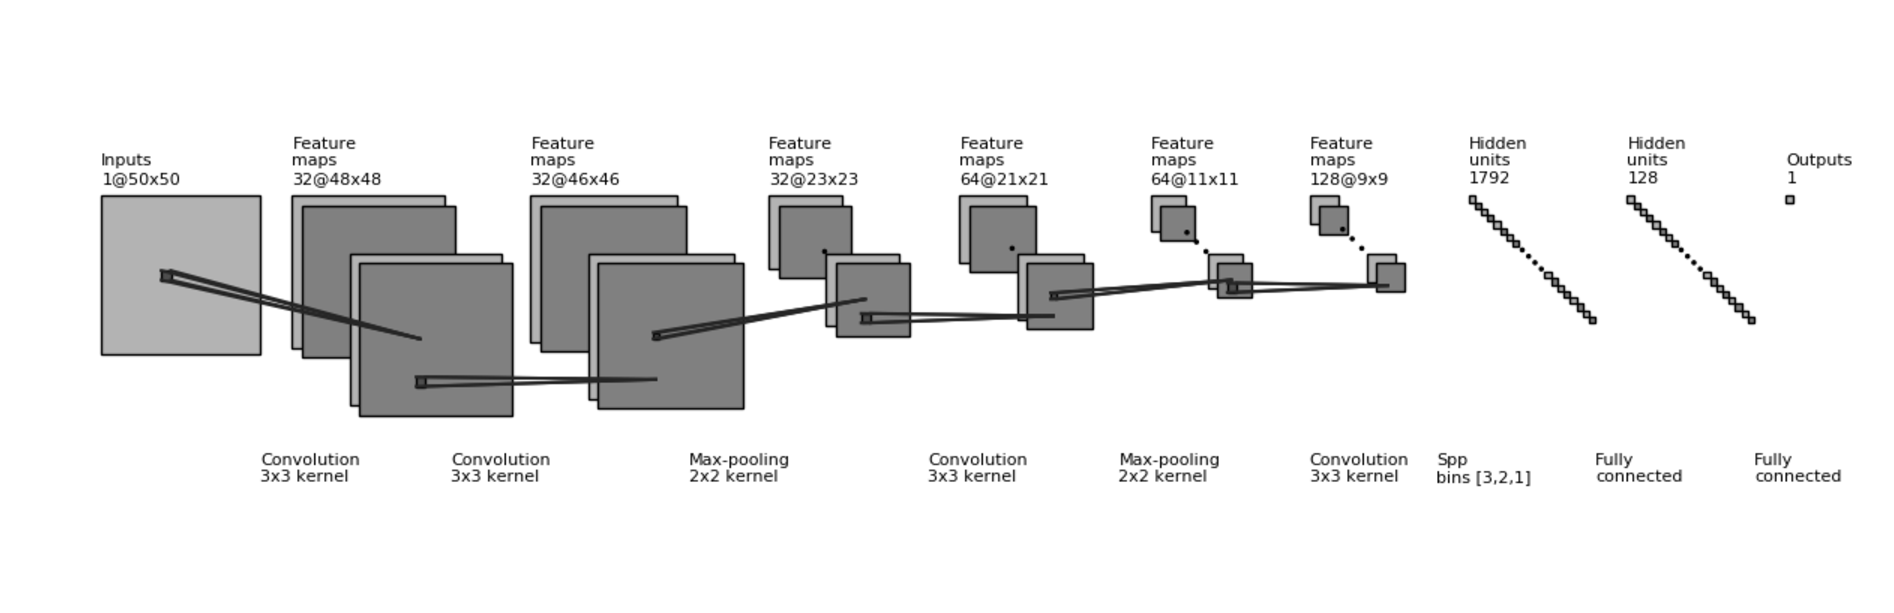
\includegraphics[scale=0.5]{eps/mynet.eps}}
    \caption{我的网络结构示意}
    \label{fig:label}
\end{figure}
spp层是使用了动态尺寸的池化核将任意尺寸的输入池化到固定尺寸的输出。首先需要一个$BINS$来决定输出的尺寸,通常会选择多个输出尺寸来获得更多的信息。如输入图片尺寸为$x \times x$,需要的输出尺寸为$n \times n$,则计算
$$ksize = \lceil \frac x n \rceil$$
$$stride = \lfloor \frac x n \rfloor$$
再利用$ksize$和$stride$做最大池化。对$BINS$中每个输出尺寸都做了最大池化后,把这些数据排成一行输出到全连接层。\cite{spp}最开始是为了实现输入不同尺寸的图片到网络中进行训练所以想使用spp,但由于tensorflow的局限,一是如果输入不同尺寸的图片,就没法使用batch,只能每次输入一个图片;二是spp需要使用图片的动态尺寸,生成动态池化核来进行池化,但tensor自带的池化函数只支持静态池化核,需要自己重写池化函数,又遇到了使用tensor写循环语句的困难。考虑到图片伸缩对本问题的影响不大,故最后改为将输入单词图片都resize到$50 \times 50$,但仍然保留spp层。尽管spp层也需要每次输入的图片尺寸相同,但如果输入图片都变为另外一个尺度,网络也不需要改动,可以直接利用原网络。这样就可以实现多尺度维度的输入来提高效果。

相对于之前的LeNet,网络深度更深,输入图片尺寸的设计也更为灵活,连续使用了两个$3 \times 3$的卷积核来代替原来的一个$5 \times 5$的卷积核则是基于VGGNet的思想。

在损失函数上,考虑到我们的问题中精确度比较重要,故在损失函数中降低了正样本的比重。原本的损失函数为
\[\mathsf{targets} \times -\log(\mathsf{sigmoid}(\mathsf{logits})) + (1 - \mathsf{targets}) \times -\log(1 - \mathsf{sigmoid}(\mathsf{logits}))\]
新的损失函数为
\[\mathsf{targets} \times -\log(\mathsf{sigmoid}(\mathsf{logits})) \times \mathsf{pos\_weight} +(1 - \mathsf{targets}) \times -\log(1 - \mathsf{sigmoid}(\mathsf{logits}))\]
其中$\mathsf{targets}$为数据的标签,正样本为1,负样本为0,我们的数据中公式图片为正样本。$\mathsf{logits}$为网络的输出,经$\mathsf{sigmoid}$后为网络预测的为正样本的概率。$\mathsf{pos\_weight}$则是我们加入的一个比重,用来调节损失函数。当我们令这个比重小于1时,若网络的输入为正样本,则损失函数更小。

\section{CTPN的启发}
\noindent

在独立做完以上工作后,查阅论文时发现在OCR领域的一些文字识别的工作。如CTPN\cite{ctpn}、CRNN等。CRNN主要做的是文字识别工作,而CTPN做的是文字检测。

CTPN做的是自然场景图象中的水平文字检测,主要是在Faster RCNN的基础上结合双向LSTM生成的模型。首先是通过VGG提取特征,将生成的feature map经过一些处理后输入双向LSTM中,生成既包含CNN学习到的空间特征,也包含LSTM学习到的序列特征的特征图。再将特征图通过类似Faster RCNN的RPN网络,获得建议文本位置(text proposals)。CTPN生成的是宽度不变的anchor,通过寻找anchor中心和高度来获得一个小尺寸的建议文本位置,如图3.2,上面是传统的RPN的输出,下面为CTPN输出的建议文本位置,可以看见一个文本有许多小宽度的建议位置,接下来只需要通过文本线构造办法,将这些连接起来形成一个文本检测框。

\begin{figure}[hp]
    \centering
    
\includegraphics[scale=0.5]{eps/rpn.eps}
    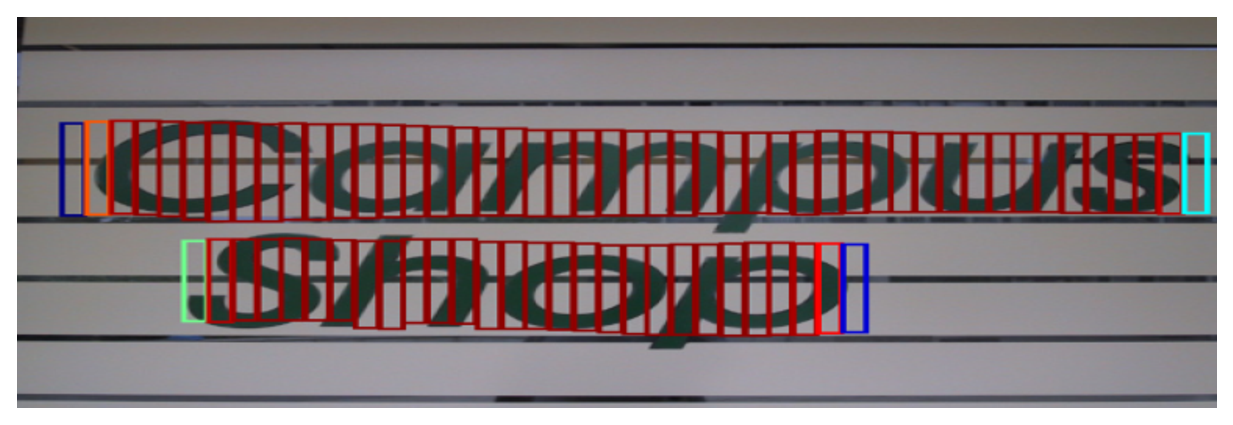
\includegraphics[scale=0.5]{eps/ctpn.eps}
    \caption{CTPN proposals}
    \label{fig:label}
\end{figure}

CTPN的工作是自然场景图象中的文字检测,用在我们的论文图片中有大材小用的样子。但是CTPN的方法给予了我一些启发。在处理单词图片时我们直接将单词图片resize到了固定长宽。单词图片长宽比例很不均匀,若直接resize到方形,原本长宽比例很大的单词和长宽比例接近1的单词就显得不对等,而公式图片的特征变化更为明显。在CTPN中并不直接检测整个文本,而是一段一段地检测文本。故在处理图像时把长宽比大于2的单词分割为两个图片,前者长宽比为1比1,后者为剩下的,递归此操作,最终得到的图片长宽比都不大于2,这样再resize损失的特征大大减少。

\section{更精确的单词切割}

数据预处理将直接影响到最终的结果,特别是文行的切割对结果影响非常大。主要原因是把行间公式和正常文行分开比较困难,而我们的数据中行间公式没有被标记为正类,故测试时网络可能将行间公式预测为正类,而降低precision。在没有进行数据平衡的测试集上,行内公式的数量远小于单词数,而行间公式的数目也不小,而且一个行间公式就会被切割为大量的单词,如果不能很好地排除掉行间公式,尽管网络实际效果很好,precision也不会太高。

首先对于文行单词分割,最大的问题在于没有处理大空白,如果空白数量比较少,则可能单词间空白和字母间空白一起被排除掉,而一行的大空白一般只有一两个,故在处理时只需要将最大的两个空白改为第三的值,然后再进行最小二乘法,就可以比较好地处理这种情况。又由于以上CTPN的启发,单词切割的精确性要求大大降低,只需要位置信息能够还原就足够了。文行分割的问题比较复杂,而且很难做到完全准确的分割。行间公式的情况比较复杂,想简单地通过几个标准把行间公式完全排除比较困难,可以尝试用机器学习去自动学习行间公式的特征从而得到更好的结果,这里只使用了由经验总结出的一些方法。

得到了用空行分割的文行后再继续进行进一步的筛选,需要使用一些指标。之前我们使用的是文行的高度、中心行和、前四分之一行和、开始行和以及结尾行和。中心行和是一个不太好的指标,只采用文行的中心行和来进行判断其准确度比较低,主要是中心行和缺乏代表性,虽然总的来说行间公式的中心行和一般比较小,但如果遇到分数线则会大大增加中心行和,而且中心行和很不稳定,波动的范围比较大。为了解决这个问题首先想的是再中心行附近一定范围内随机取一行来求和来作为标准,这种方法十分不稳定,甚至会导致较大的误差,不能保证结果。最后使用的是文行所有行和的平均,成为平均行和,平均行和比较稳定,区分度也比较好,相应的前四分之一行和也使用平均行和。至于行和高度更是一个极不稳定的指标,尽管有的行间公式高度很大,但有的则与目标文行没有差别,甚至有的目标文行如果含有一些公式符号则比行间公式的高度还要大。因此在筛选时的主要标准是平均行和,高度只作为一个辅助标准。同时为了更精确,求高度的分界线时也使用最小二乘法。平均行和和前四分之一行和相比,后者又具有更好的区分性,因为行间公式开头一段通常是空白,因此主要标准为前四分之一行和,使用平均行和和高度来进行辅助。这样调整之后效果有了很大的改进,但仍然无法完全排除行间公式,故测试结果仍然比实际要差,所以我们将通过直接查看在论文图片上的效果来人工评估一下模型效果。

\section{网络训练结果比对}
\noindent

测试结果评估采用了4个指标,accuracy、precision、recall、F1 Measure。TP为预测正确的正类,FP为预测错误的正类,TN为预测正确的负类,FN为预测错误的负类。accuracy为所有图片预测正确的概率,precision为预测为正类的图片中预测正确的比例,recall为所有正类中被预测正确的比例,F1为precision和recall的调和平均。
\[accuracy = \frac {TP + TN} {TP + FP + TN + FN}\]
\[precision = \frac {TP} {TP + FP}\]
\[recall = \frac {TP} {TP + FN}\]
\[F_1 = \frac {2 TP } {2 TP + FP + FN}\]
为了能够查看在实际图片上的效果,可使用文件formula\_find.py。这个文件将输入的图片先做空白边框去除和单词分割,然后将图片依次传入训练好的网络模型中,得到结果后再使用每张图片的位置信息在原图像上进行标注,对于被分割的公式,在重建时直接将相邻的被预测为公式的单词合并起来,然后用红框标注。

Os使用过采样的数据,训练数据571029张单词图片,测试图片12637张。Us为使用欠采样的数据,训练数据404383张单词图片,测试图片12637张。以上两种没有使用方形单词分割,Sq为使用了方形单词分割作为训练和测试集,训练数据465974张单词图片,测试图片22391张。Us与Sq使用的训练原始数据,即没有经过预处理的数据相同,但方形单词分割会得到更多的图片。Os因为过采样,所以原始数据比后两者要少。

\begin{figure}[hp]
    \centering
    \begin{tabular}{cccc}
    \toprule
    Set& 训练集& 测试集\\
    \midrule
    Os& 571029& 12637\\
    Us& 404383& 12637\\
    Sq& 465974& 22391\\
    \bottomrule
    \end{tabular}
    \caption{各数据集数据量}
\end{figure}

三种模型都以100大小的batch进行5000次训练,结果发现Sq各方面优于Us,Us优于Os。但Os结果实际上已经还不错,故提升的幅度比较小。

\begin{figure}[hp]
\centering
\begin{tabular}{ccccc}
\toprule
Set& accuracy& precision& recall& F1\\
\midrule
Os& 0.9901& 0.9316& 0.9987& 0.9640\\
Us& 0.9904& 0.9343& 0.9975& 0.9648\\
Sq& 0.9946& 0.9418& 0.9995& 0.9698\\
\bottomrule
\end{tabular}
\caption{测试集上结果}
\end{figure}

\section{实际效果演示}
\noindent

三个网络的实际表现都已经非常不错,实际准确率非常高,故接下来主要演示一下结果不准确的部分及其原因。首先是由于文行分割导致的问题,有些过短的行被排除了,如果其包含公式就不会被检测,这样的情况如图。然后是一些公式符号单独成行,但这一行也被排除了,如图。还有有的行间公式没有无法排除掉,造成如图的情况。
\begin{figure}[hp]
    \centering
    \begin{subfigure}[b]{\linewidth}
    \centering
    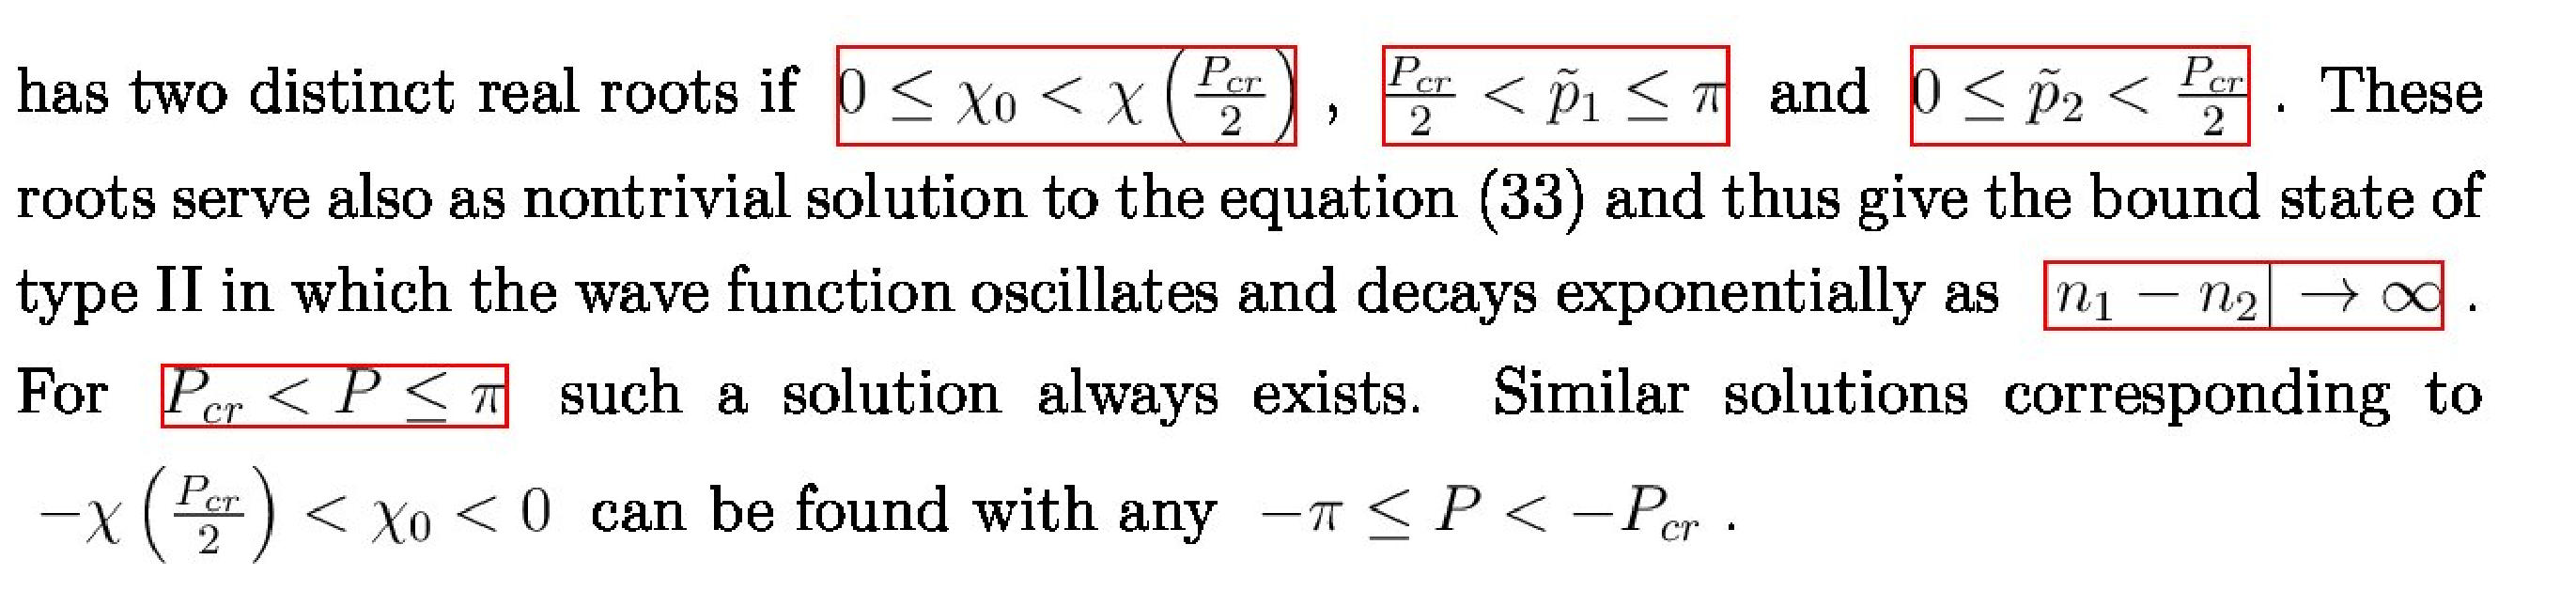
\includegraphics[scale=0.3]{eps/a11.eps}
    \caption{\label{fig:fig1}}
    \end{subfigure}

    \begin{subfigure}[b]{\linewidth}
    \centering
    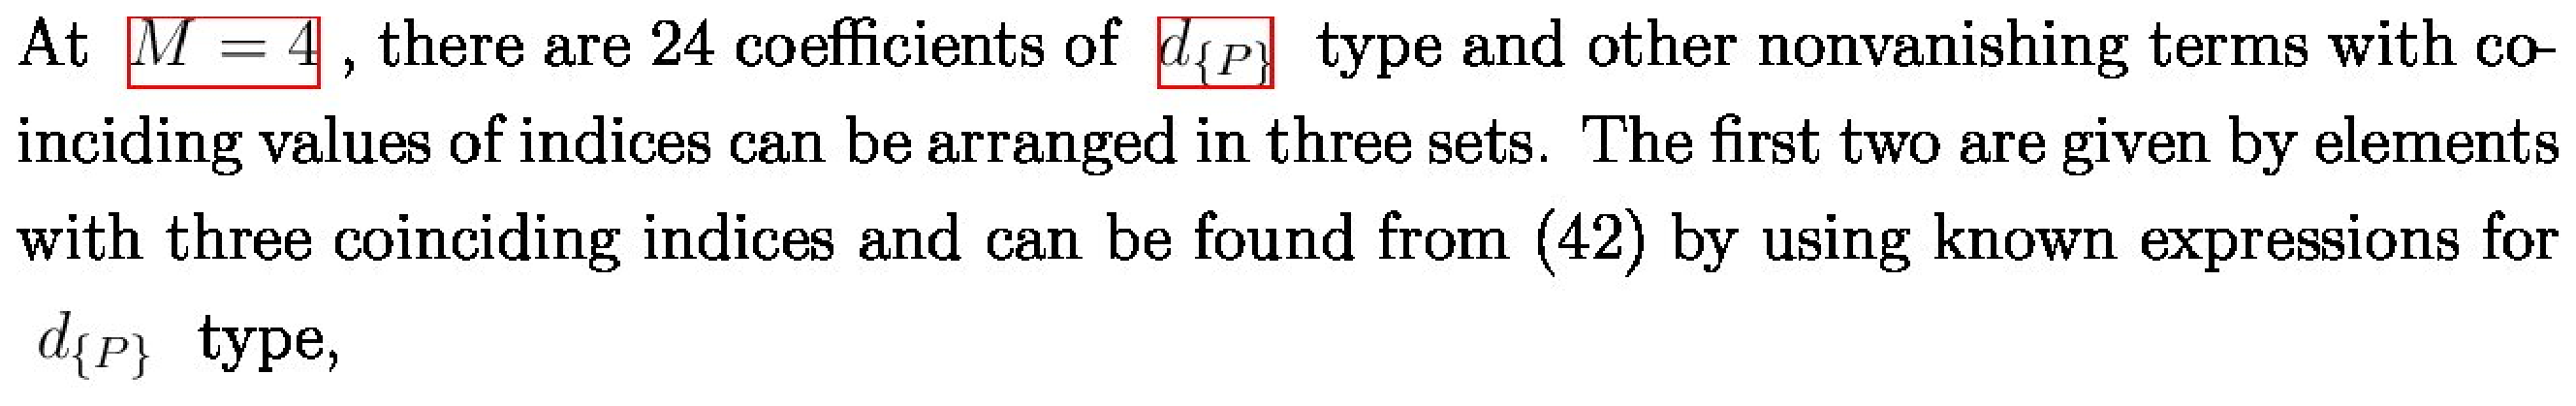
\includegraphics[scale=0.3]{eps/a12.eps}
    \caption{\label{fig:fig2}}
    \end{subfigure}

    \begin{subfigure}[b]{\linewidth}
    \centering   
    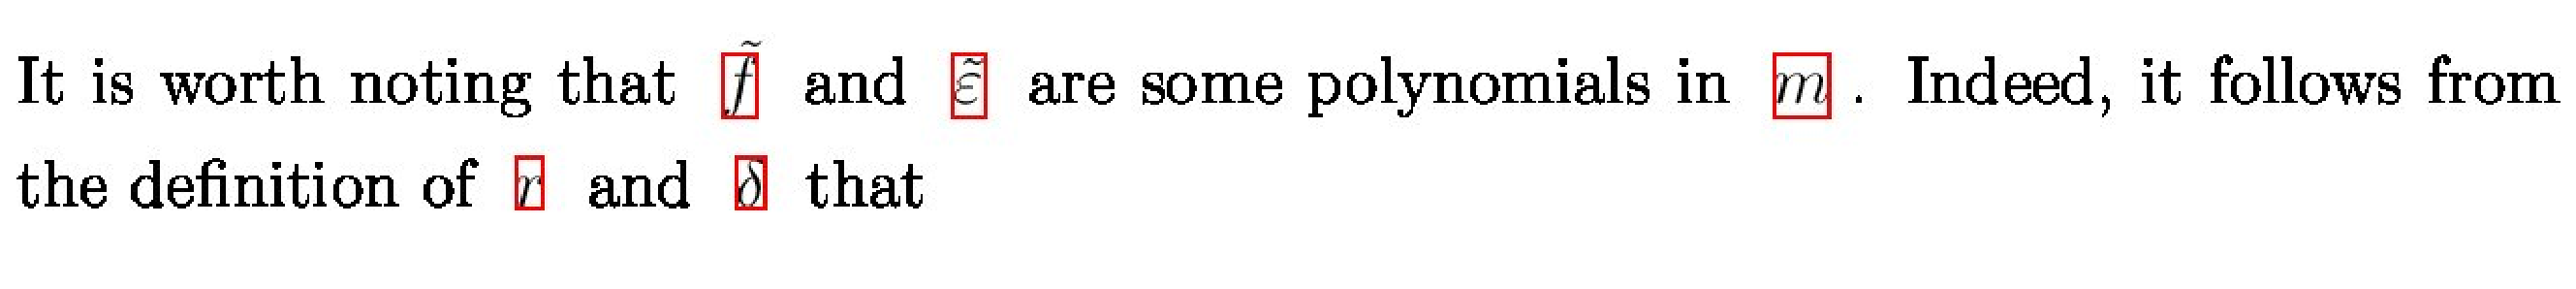
\includegraphics[scale=0.3]{eps/a13.eps}
    \caption{\label{fig:fig3}}
    \end{subfigure}

    \begin{subfigure}[b]{\linewidth}
    \centering 
    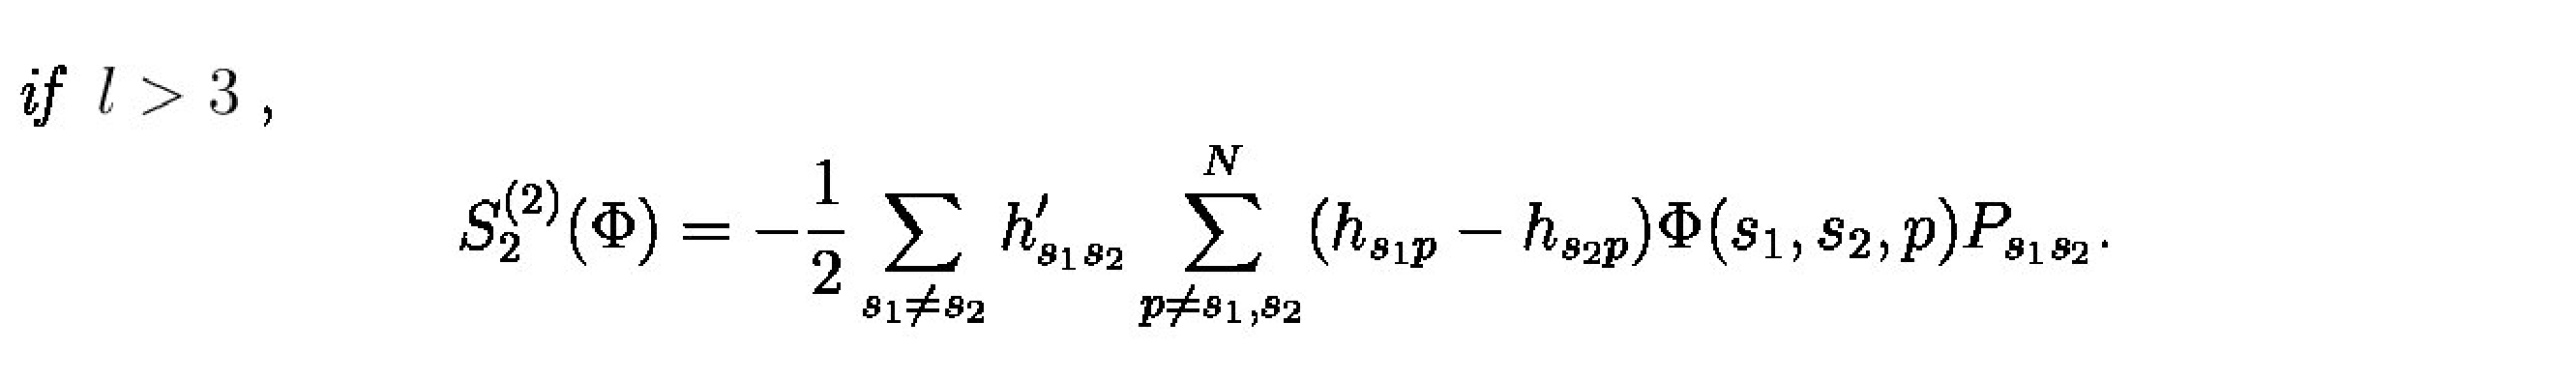
\includegraphics[scale=0.3]{eps/a14.eps}
    \caption{\label{fig:fig4}}
    \end{subfigure}

    \begin{subfigure}[b]{\linewidth}
    \centering 
    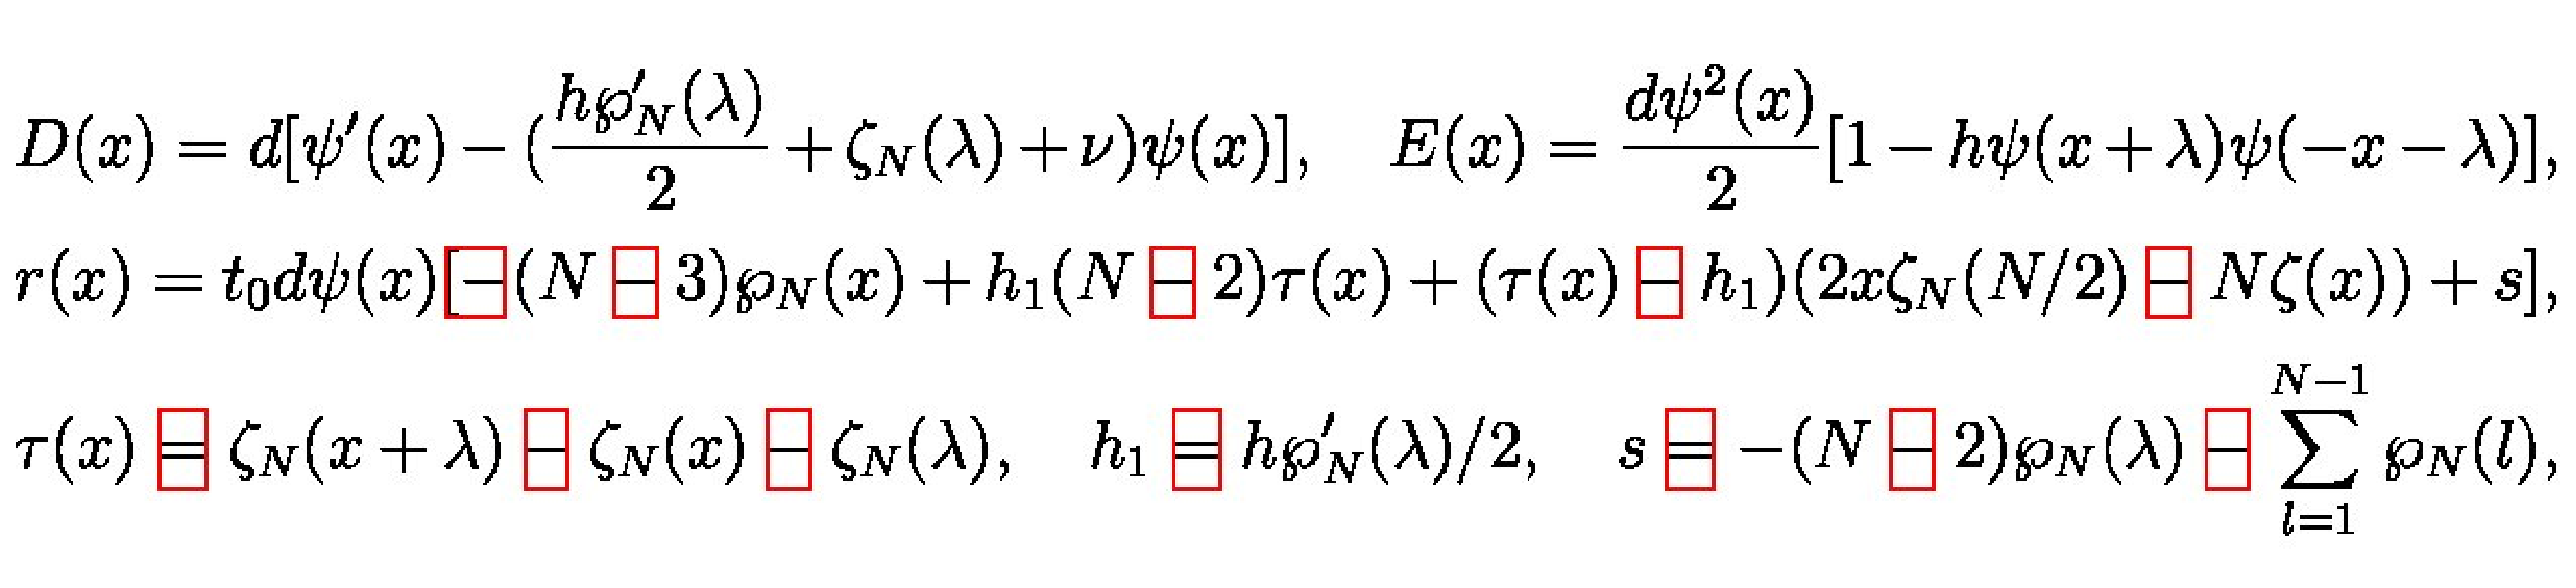
\includegraphics[scale=0.3]{eps/a15.eps}
    \caption{\label{fig:fig5}}
    \end{subfigure}

    \caption{文行分割导致的问题}
    \label{fig:label}
\end{figure}

\begin{figure}[hp]
    \centering
    \begin{subfigure}[b]{\linewidth}
    \centering
    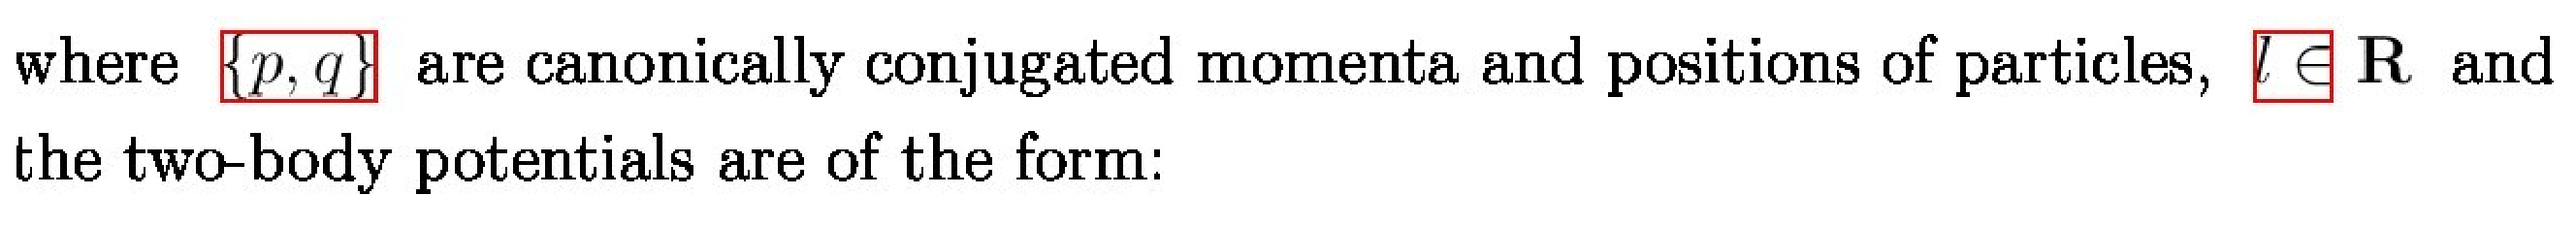
\includegraphics[scale=0.3]{eps/a21.eps}
    \caption{\label{fig:fig1}}
    \end{subfigure}

    \begin{subfigure}[b]{\linewidth}
    \centering
    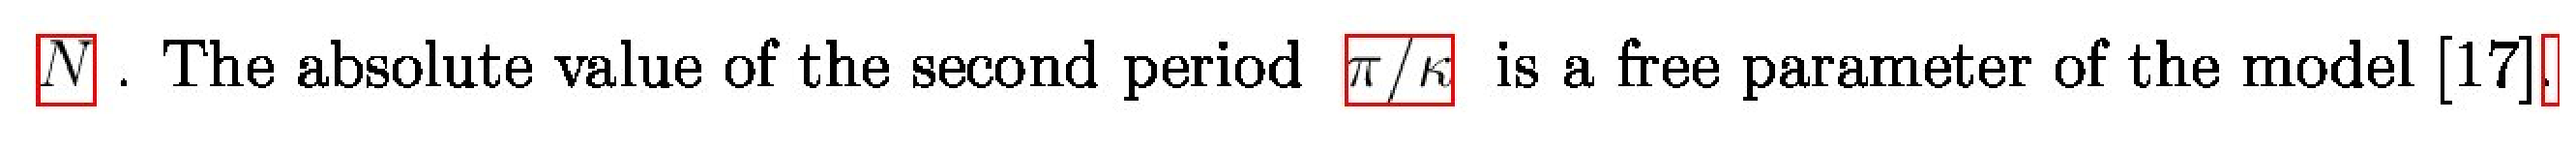
\includegraphics[scale=0.3]{eps/a22.eps}
    \caption{\label{fig:fig2}}
    \end{subfigure}

    \begin{subfigure}[b]{\linewidth}
    \centering
    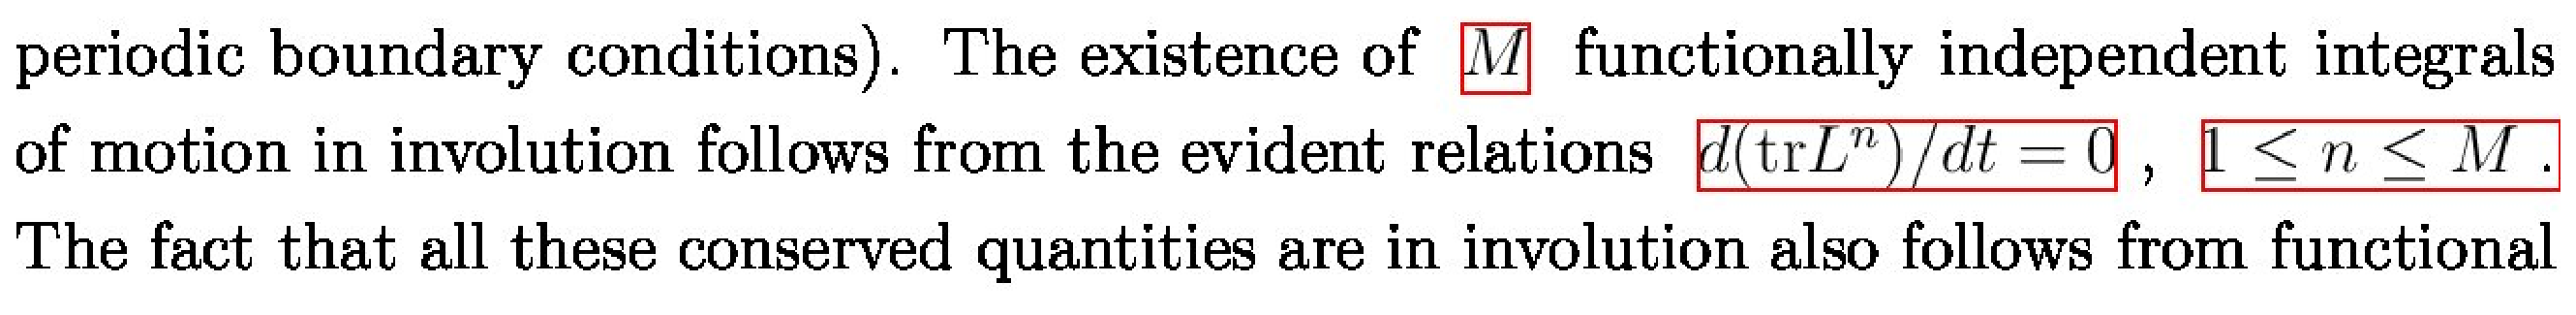
\includegraphics[scale=0.3]{eps/a23.eps}
    \caption{\label{fig:fig2}}
    \end{subfigure}

    \begin{subfigure}[b]{\linewidth}
    \centering
    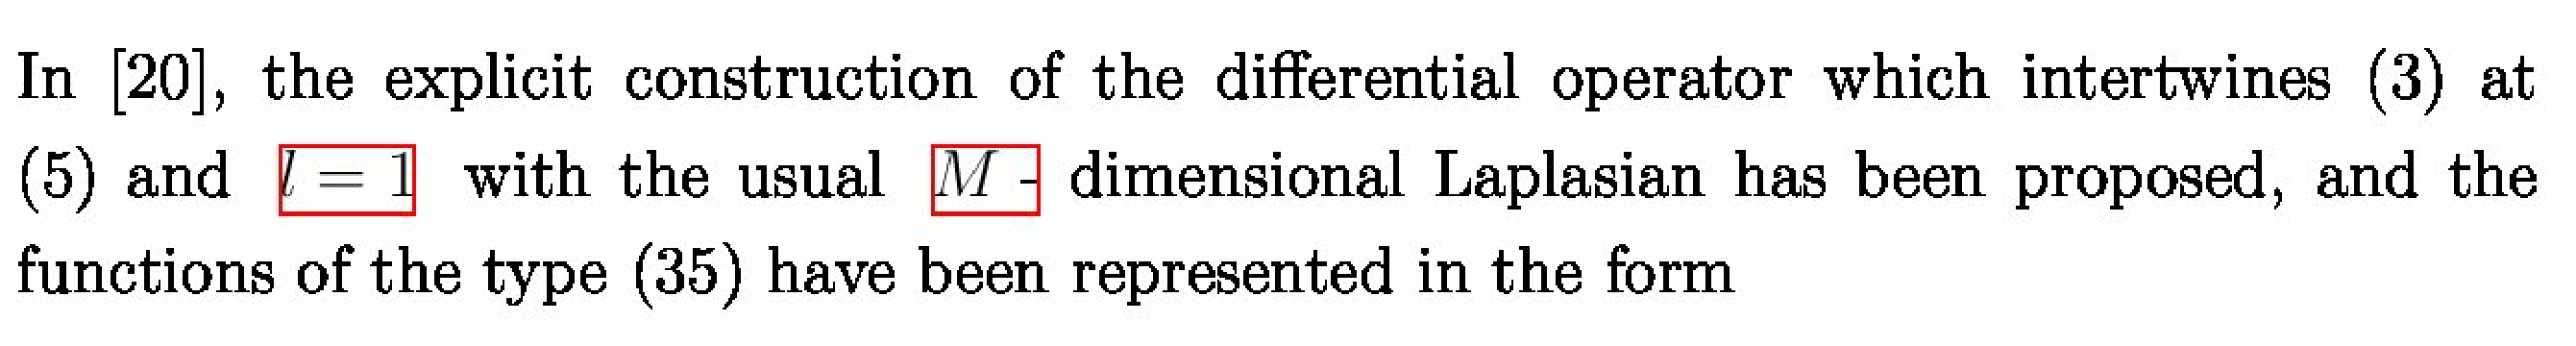
\includegraphics[scale=0.3]{eps/a24.eps}
    \caption{\label{fig:fig4}}
    \end{subfigure}

    \caption{网络学习的问题}
    \label{fig:label}
\end{figure}


\begin{figure}[hp]
    \centering

    \begin{subfigure}[b]{\linewidth}
    \centering
    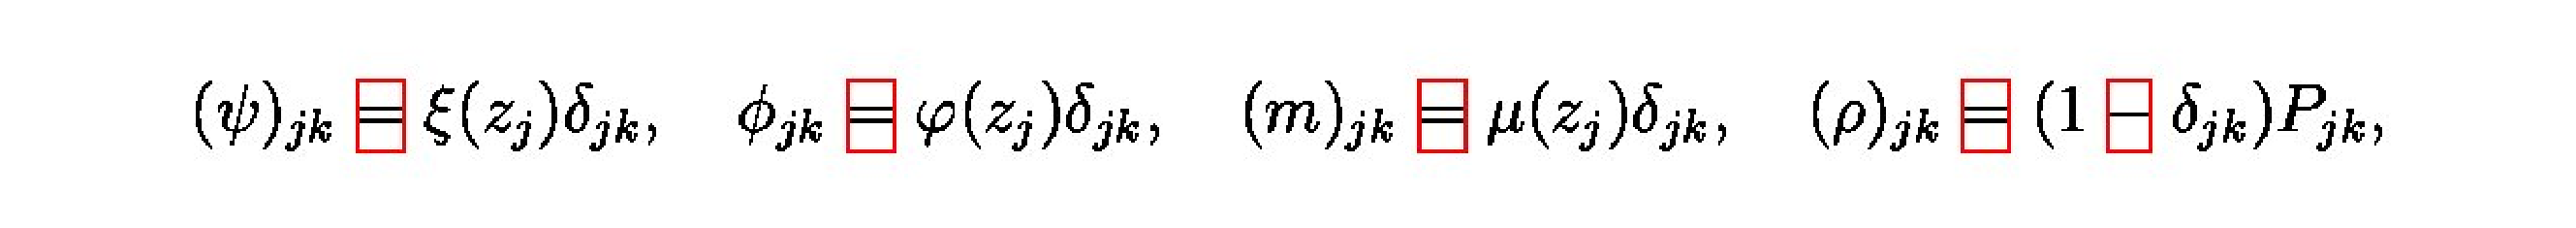
\includegraphics[scale=0.3]{eps/os1.eps}
    \caption{\label{fig:fig1}}
    \end{subfigure}

    \begin{subfigure}[b]{\linewidth}
    \centering
    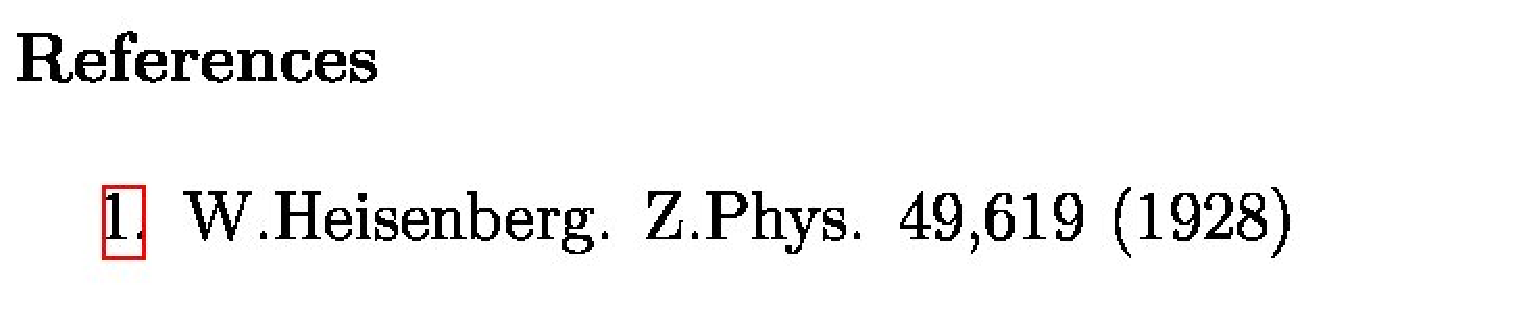
\includegraphics[scale=0.3]{eps/os2.eps}
    \caption{\label{fig:fig2}}
    \end{subfigure}


    \caption{Os的问题}
    \label{fig:label}
\end{figure}

\begin{figure}[hp]
    \centering

    \begin{subfigure}[b]{\linewidth}
    \centering
    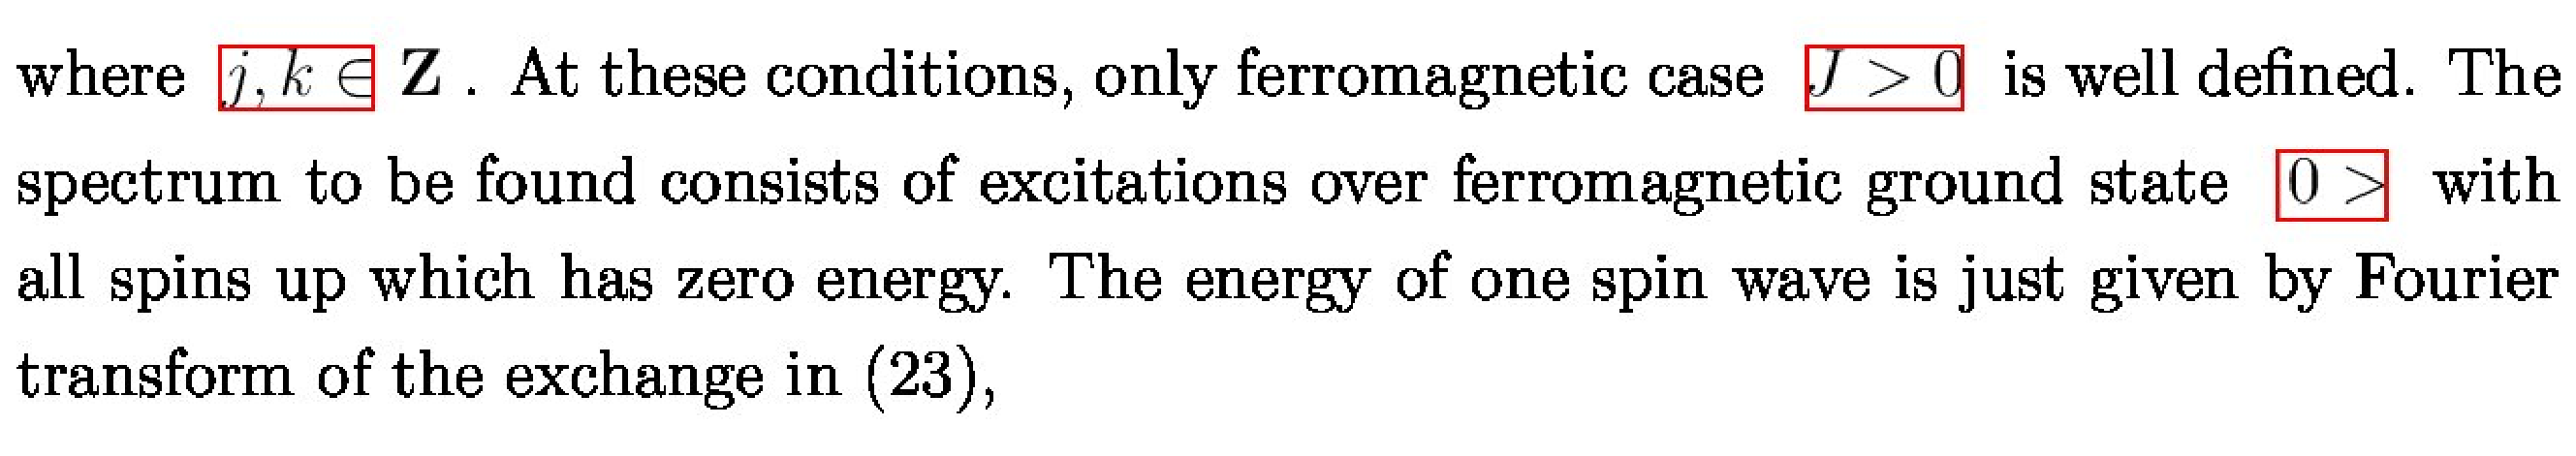
\includegraphics[scale=0.3]{eps/us1.eps}
    \caption{\label{fig:fig1}}
    \end{subfigure}

    \begin{subfigure}[b]{\linewidth}
    \centering
    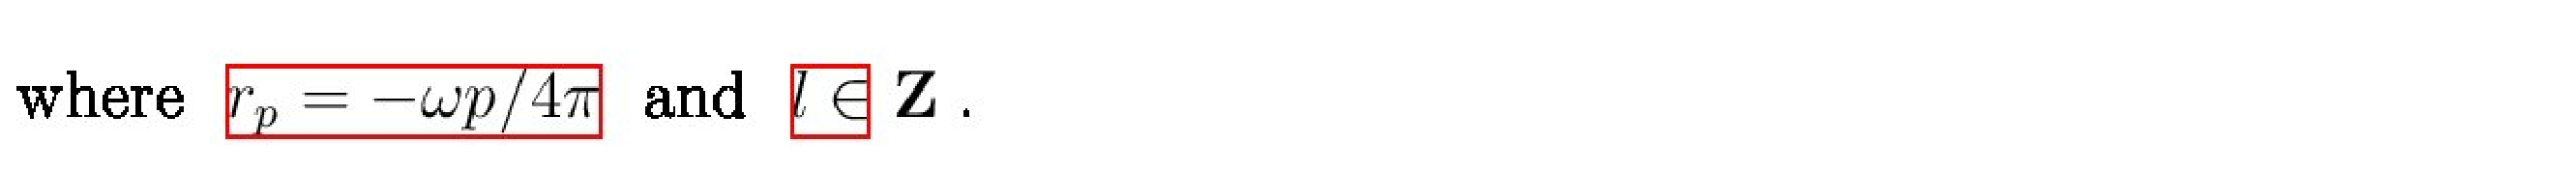
\includegraphics[scale=0.3]{eps/us2.eps}
    \caption{\label{fig:fig2}}
    \end{subfigure}

    \begin{subfigure}[b]{\linewidth}
    \centering
    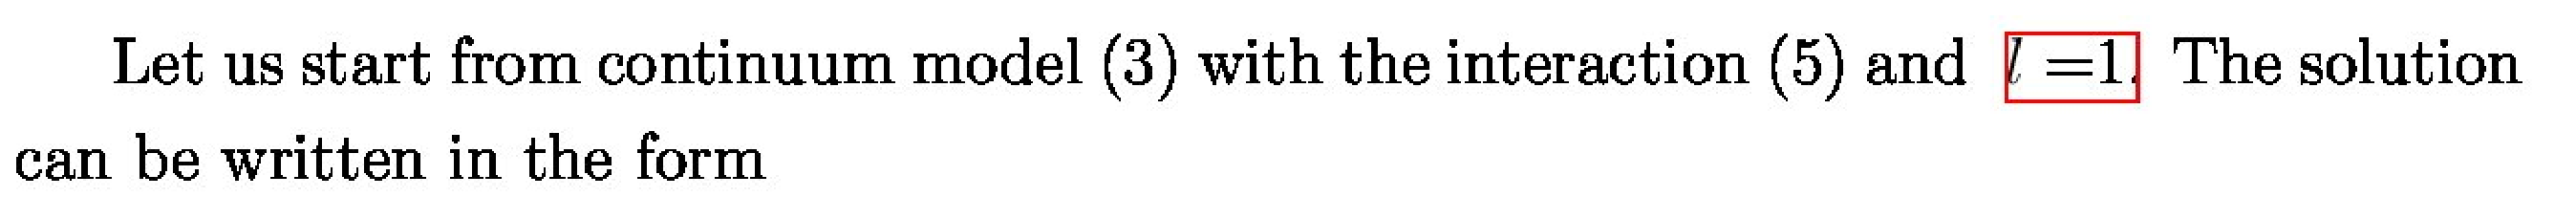
\includegraphics[scale=0.3]{eps/us3.eps}
    \caption{\label{fig:fig3}}
    \end{subfigure}


    \caption{Us的问题}
    \label{fig:label}
\end{figure}

\begin{figure}[hp]
    \centering

    \begin{subfigure}[b]{\linewidth}
    \centering
    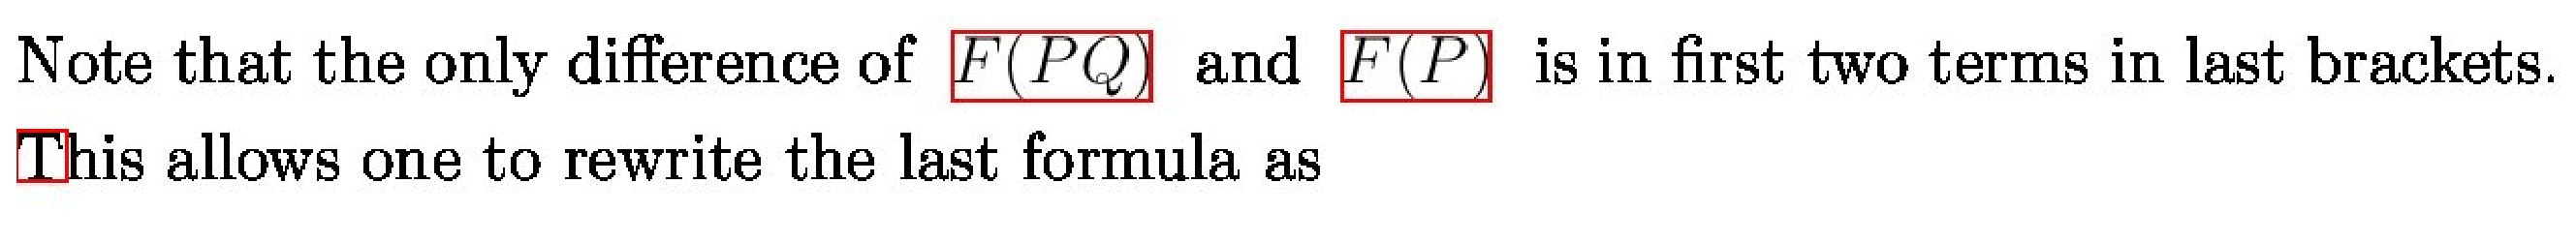
\includegraphics[scale=0.3]{eps/sq1.eps}
    \caption{\label{fig:fig1}}
    \end{subfigure}

    \begin{subfigure}[b]{\linewidth}
    \centering
    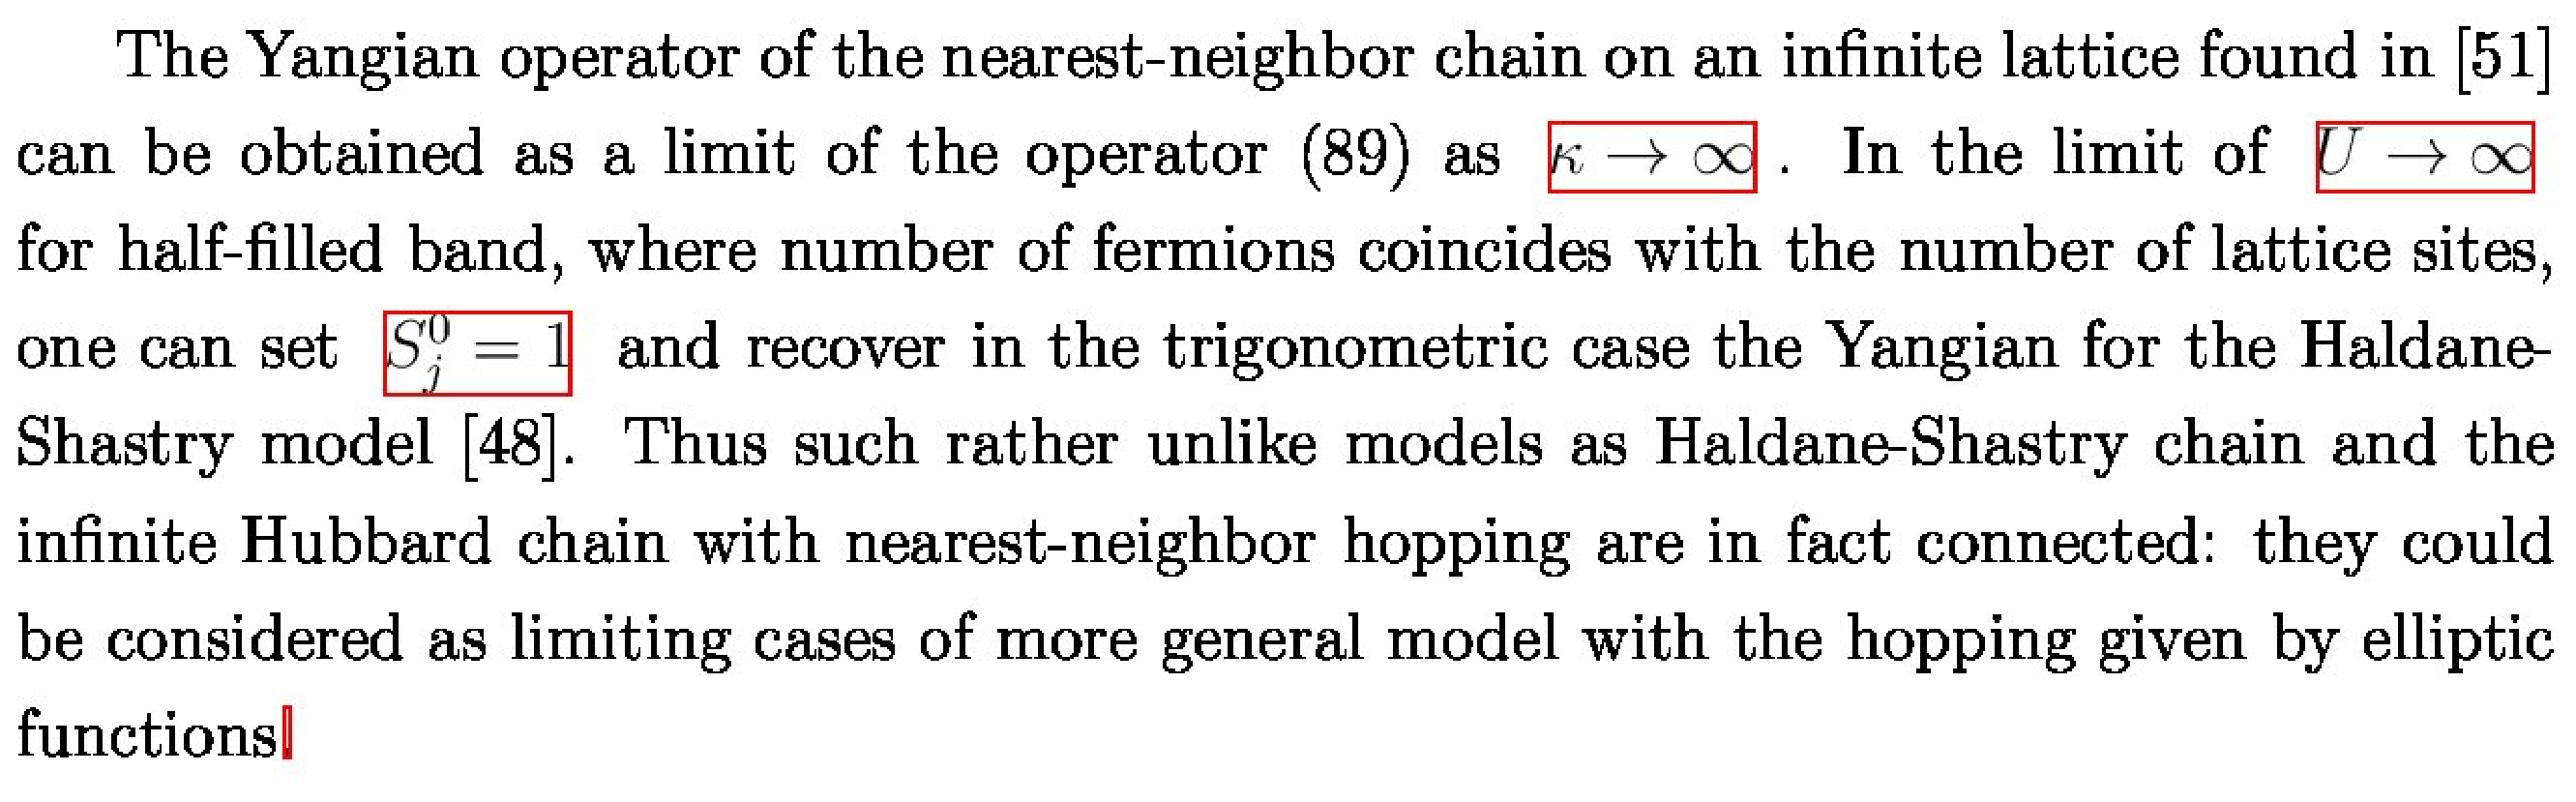
\includegraphics[scale=0.3]{eps/sq2.eps}
    \caption{\label{fig:fig2}}
    \end{subfigure}

    \begin{subfigure}[b]{\linewidth}
    \centering
    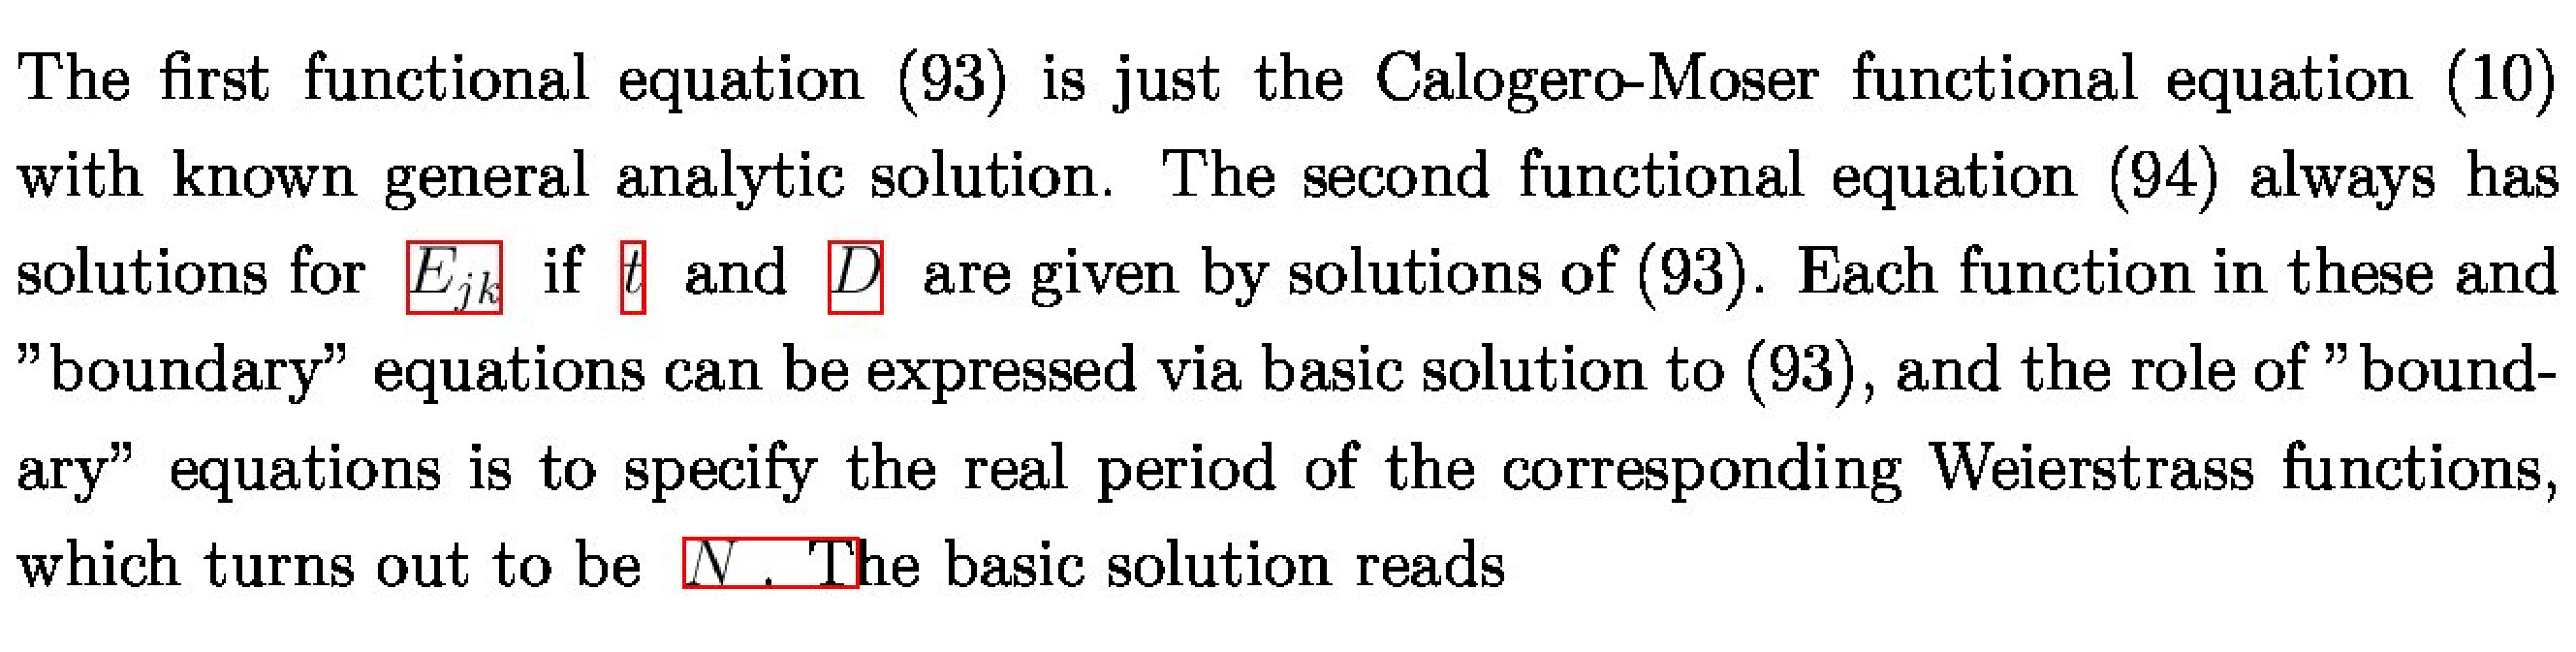
\includegraphics[scale=0.3]{eps/sq3.eps}
    \caption{\label{fig:fig3}}
    \end{subfigure}

    
    \caption{Sq的问题}
    \label{fig:label}
\end{figure}